\documentclass[10pt]{article}

\usepackage{url}
\usepackage{graphicx}
\usepackage{color}
\usepackage{amsmath}
\usepackage{hyperref}
\usepackage{fullpage}
\usepackage{natbib}

% Code for changing the color of the hyper-references
\hypersetup{
    colorlinks,
    citecolor=blue,
    filecolor=black,
    linkcolor=blue,
    urlcolor=blue
}

\title{Project Waste}
\author{Avikalp Kumar Gupta}
\date{\today}

\begin{document}
\maketitle

\tableofcontents

\pagebreak

\begin{abstract}



\end{abstract}

\section{Problem Statement}

We want to solve the problem of responsible waste disposal for the cities of India. We want Indian cities to look clean and keep its citizens healthy and productive for the betterment of the country. Our aim is to come up with a sustainable solution for the same. The scope of this particular project is currently restricted to the city called \emph{Bengaluru}, capital city of the Karnataka state. 

\section{Introduction}

In India, people are too particular about cleanliness. Their clothes, their houses, their food, everything must be clean. But they make efforts only at micro-levels. In the discussion of solid waste disposal, the job of Indians ends as soon as the garbage is outside the door of their house. They do not realize that the waste that is lying right outside their house still makes their house look filthy and will still make their children sick. 

Human activities generates all forms of waste - solid, liquid (effluents) and gaseous (pollution). In this project, we are focussing the solid waste generated by human activities. This solid waste can be categories in 3 broad categories - dry waste, wet waste and hazardous waste. Wet waste is the more organic readily bio-degradable waste, which mainly consists of the by-products of food preparation and the left-over food.

The BBMP has defined 6 stages of solving the problem of waste management \citep{BBMP:SWMOverview}:
\begin{enumerate}
\item Collection of waste
\item Segregation of Waste
\item Intra-city activies (like sweeping the roads etc.)
\item Storage of waste
\item Transportation of the waste
\item Processing of waste
\end{enumerate}
Although $6^{th}$ stage of this pipeline is the most crucial in terms of responsible solid waste management, our focus will be on the first 5 stages (except maybe the $3^{rd}$ stage). We hope to be able to partner with some companies working on the processing of different kinds of wastes to manage our collections.

Bulk waste generators are defined by BBMP as \emph{``Bulk Generators includes domestic generators-apartments complexes in more than 50 units and institutional and commercial bulk generators who produce more than 10 kg of Municipal Solid Waste"}. Among the bulk waste generators in the city are 15,000 apartment complexes. Any establishment which generates more than 100 kg of wet waste per day is defined as a bulk waste generator. Apartment complexes with more than 50 flats have been identified as bulk generators. Other bulk generators include restaurants, hotels, and choultries\citep{BangaloreMirror:bulk_waste_generators}. \href{http://bbmp.gov.in/documents/10180/2201631/Approved+Vendor+List+with+note+for+Website+21-06-2016.pdf/34567fdf-8d69-4b12-8440-9475ba4a0567}{This document on BBMP's website} lists the various options available to thse bulk waste generators to handle those huge quantities of waste that they produce.

But for the small waste generators, like the individual households, it very costly and difficult to dispose their waste responsibly. The BBMP does collection of the garbage from a lot of them and from the streets as well, but probably this waste is not processed. It probably is openly dumped into nearby rural areas, where it degrades the soil and troubles the life of the residents. At least before December 2014, a lot of Bengaluru's garbage was being dumped at Mandur \citep{BangaloreMirror:bulk_waste_generators}.
\textcolor{red}{We still have to verify whether this is still happening, or has the situation changed. We have some experiments in mind for the same.}


%-----------------------------------------------------------------%
%------------------------ Section Boundary -----------------------%
%-----------------------------------------------------------------%

\section{Status Quo}



\subsection{BBMP: Bruhat Bengaluru Mahanagara Palike}

The Municipal Corporation of Bengaluru, i.e. the BBMP, has been active in the last decade in solving the waste management problem of the city. \cite{BBMP:SWMOverview} gives a good overview of the arrangements that the BBMP has planned for managing the city's waste.

\subsubsection{Collection and Segregation of Waste}

According to \cite{theHindu:segregation_at_source_31Jan2017}, BBMP had made it mandatory to segregate waste at source from February 2017. From this date, the waste collectors, better known as \textit{Pourakarmikas}, are entitled to refuse to collect mixed waste. BBMP is implementing this plan by collecting wet waste and sanitary waste everyday, but the dry waste will only be collected twice a week (the two days of collection will be specific to each ward).
There are fines for refusing to segregate the waste, which increases with persistance to not comply. If someone refuses to pay the fine, the amount will be added to the property tax.

Before this drive by the BBMP, the various other efforts by BBMP had managed to get about 35\% of the city to segregate its waste, and with this drive, it is aiming to increase this number to 60\%.

\#update: $18^{th}$ April, 2017

According to \cite{ToI:segregation_at_source}, on a single day (April 4, 2017):
\begin{itemize}
	\item Of the total waste of 4039.76 tonnes, 2057.03 tonnes were segregated at source
	\item In all, 1677.65 tonnes of wet waste and 362.65 tonnes of dry waste were segregated at source
\end{itemize}
The city has collected over 20 tonnes of sanitary waste separately in the first week of April (2017).
 "In some places, there are complaints that pourakarmikas mix up waste even though it had been segregated by households. We're looking into these problems. Low quality plastic and mixed waste are still going to quarries. Collection and disposal have been big challenges," said Sarfaraz Khan.


\subsubsection{Intra-city activities}

\subsubsection{Storage and Transportation of waste}

\subsubsection{Processing of waste}

\subsection{Hasiru Dala}

The following describes the vision of Hasiru Data \citep{HasiruDala:home}:

\begin{itemize}
\item We want waste workers to participate in society, free from discrimination.
\item We organize waste pickers so that they can fight for their rights.
\item We conserve our natural habitats
\item We strive to improve working conditions.
\end{itemize}

Hasiru Dala has another sibling company called ``Hasiru Dala Innovations". Here is what its website has to say about itself \citep{HasiruDalaInnovations:about}:

``Hasiru Dala Innovations is a social enterprise committed to creating predictable livelihoods for wastepickers through providing total waste management, urban gardening services and products for sustainable living. All our initiatives are designed to enable a circular economy that enhances the lives, be it a wastepicker or a resident, it touches."

\subsection{Saahas Zero Waste}

Here is what Saahas Zero Waste's website says about itself \citep{SaahasZeroWaste:about}:

``Saahas Zero Waste (SZW) is a socio-environmental enterprise that believes in a circular economy, where all waste is converted to resources. Registered in 2013, SZW is recognised as a Startup by the Department of Industrial Policy and Promotion, Government of India.

At Saahas Zero Waste, we leverage Nature, People and Technology to holistically manage waste. Through the Zero Waste Programme we operate on-site solutions for bulk waste generators including tech parks and residential complexes. For smaller waste generators, we offer holistic waste management which includes collection and process at our units, Kasa Rasa. Our focus is to help our clients become zero waste entities with emphasis on segregation at source.

In the Extended Producer Responsibility (EPR) program, we partner with packaging companies and E-Waste producers to develop and implement a reverse logistics mechanism that facilitates in bringing back large volumes of post-consumer waste into the recycling chain.

As a part of the closing the loop initiative, SZW offer products made from waste including compost and a range of other recycled products like roofing sheets, chipboards, stationary items.

With over 15 years of domain expertise and a perfect blend of senior team of experts and an excited young team, SZW currently manages 25 Tons of waste per day across Bangalore, Chennai and Hyderabad. SZW also supports livelihood at the base of the pyramid for our field staff with emphasis on health and safety."

\subsection{Daily Dump}

Daily Dump is a design led brand - a pioneer in designing and building products and services for decentralized waste management in homes, communities, offices and public spaces \citep{DailyDump:about}. Its range of segregation products, composters, books, services and more, reflects its mission to enable everyone to harm less.

On the site, one can find everything one needs to understand how waste is really a resource and to start a journey of making the world safer, cleaner and cooler! 
Daily Dump is a brand of PBK Waste Solutions Pvt Ltd.

\subsection{Encashea}

Here is what Encashea's website says about itself \citep{Encashea:about}:

``Welcome to EnCashea, an Online Place to Sell Your Scrap. Do you want to earn cash by selling your scrap online? If yes then you are at the right place. We intend to make selling scrap so much fun while ensuring safe and environment-friendly disposal of all types of scrap and recyclable material.

\begin{description}
\item[I am an individual:] If you have collected paper, books \& magazines, plastics, e-waste or household metal items in your house, then you don't need to go out to search for a kabadiwala to sell your scrap or unused stuff. You can do it from your home in an easy and convenient way. Just go to Encashea and sell scrap, metals, old newspapers and other electronic waste items directly from our website or mobile application.
At EnCashea, you will save lots of your time. We collect recyclable scrap, old newspapers, electronic wastes, old plastics, metals and other scrap materials from your doorstep and ensure they remain properly segregated and don't end up in landfills.
At EnCashea, you can sell your scrap and other unused materials in just a few clicks and get handsome money by selling your waste that other Raddiwalas cannot offer you. You can check our rates here.
Check our rate list and schedule an pickup with EnCashea now!
\item[I represent a company/office/institute:] EnCashea provides Scrap Collection and Recycling Services for institutions of all sizes. If you are an office, school or college or a company who want recyclables to be picked-up from your place, with professional services, proper invoicing and best pricing get in touch with us by filling up the form provided here."
\end{description}

\subsection{The Ugly Indian}

Here is what the Ugly Indian's website says about itself \citep{TheUglyIndian:about}:

``We are a group of Ugly Indians (the number is growing everyday) who feel strongly about the state of visible filth in our cities.\\
Our philosophy can be described simply as: \textbf{Kaam chalu mooh bandh. Stop Talking, Start Doing.}\\
We believe in direct action, with a common-sense problem-solving approach. We do not finger-point or blame the system. We aim to make a change from within - one that sustains because everyone wants it and is comfortable with it.\\
We believe that there is no magic wand, or silver bullet, to solve India's civic problems. We are realists, and accept that many of India's problems are hard to solve even if the government and public work closely together and money was freely available.\\
Of our many civic problems, we view the problem of visible filth on our streets as a behaviour and attitude problem that can be solved in our lifetime (or rather, this month). This can be achieved without spending money or changing legislation or systems. It requires coming up with smart ideas to change people's rooted cultural behaviour and attitudes. And making sure those ideas work.\\
Some of our guidelines are:
\begin{enumerate}
\item No lectures, no moralising, no activism, no self-righteous anger.
\item No confrontation, no arguments, no debates, no pamphlets, no advocacy.
\item Dont step on anyones toes, dont take sides in any ideological debates.,
\item Support existing systems and improve their effectiveness for the greater good.
\item Basically, get real. Treat everyone with sincerity, respect and dignity first, and the greater good will be an outcome.
\end{enumerate}
We feel a 'solution' is a real solution only if:
\begin{enumerate}
\item It sustains in the public street for at least 90 days.
\item With no supervision.
\item Is low-cost (ideally free) and easy to implement and replicate
\item Changes the behaviour and attitudes of all concerned
\item Creates minimal change in the daily actions of everyone concerned
    (nobody should lose a job, lose a source of income, or get seriously
    inconvenienced - because it takes only one Ugly Indian to undo the
    good work of a hundred others).
\end{enumerate}

We have chosen to remain anonymous as the names and identities of specific individuals are not important. What matters is visible results. And any visible result in the public space needs the support of hundreds of actors (the community). One Ugly Indian in each community can, and must, take the first step - but unless the community responds positively, that step will not produce results.\\
This project is as much about carrying the community along (or as is fashionable to say -being inclusive) as about coming up with smart ideas that assist the process of change."

The Ugly Indian works on the \emph{Broken Windows Theory}. They clean a spot and leave it. Once a spot is clean, it is more likely to stay clean.


\subsection{Citizengage}

Text to be added from http://citizengage.co/index.html and videos on their facebook page: https://www.facebook.com/citizengage/?fref=nf in which they have talked about their company in conferences.
%-----------------------------------------------------------------%
%------------------------ Section Boundary -----------------------%
%-----------------------------------------------------------------%

\section{Related Work}

\subsection{Kuppathotti}

Kuppathotti.com intends to help out busy people to throw away and get money for their pile of house hold junk like old newspaper, milk cover, broken things and plastic wastes etc., at door step. It avails this service upon the request sent to my bin. My service is not only for individuals but also for the organizations who find themselves deluged with a mountain of paper \citep{Kuppathotti:home}.

\begin{figure}
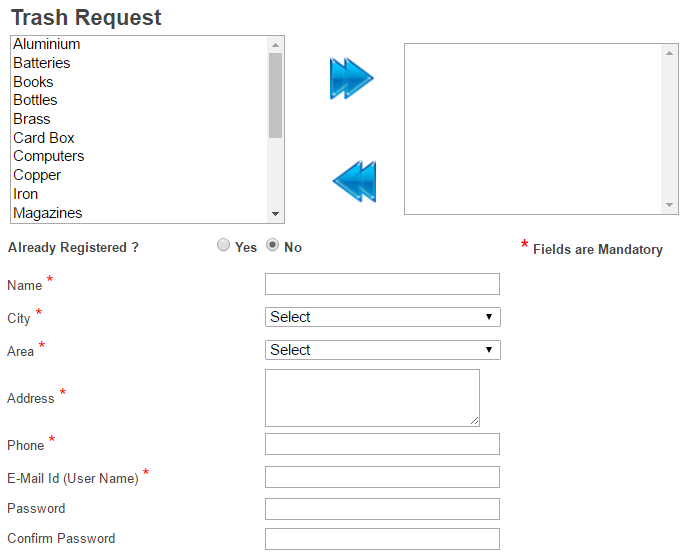
\includegraphics[width=\columnwidth]{images/Kuppathotti_trashRequest}
\caption{Trash request for Kuppathotti \citep{Kuppathotti:home}}
\label{Kuppathotti_trashRequest}
\end{figure}

Kuppathotti offers its service in the following manner:
\begin{enumerate}
\item There is form to send it a "Trash request", which takes details of the waste items that the user wants to sell along with the user's details like name \& address (see figure \ref{Kuppathotti_trashRequest}).
\item Kuppathotti will call to confirm the user's availability and will reach the address.
\item \textcolor{red}{(I do not understand this point - but it is listed in the website):} The user is contacted by Kuppathotti's suppliers.
\end{enumerate}

\subsection {Paperman}

Paperman \textcolor{red}{operates in Chennai and has already recycled more than 170 tonnes of trash}. It collects recyclables like used paper, plastic, metal, glass etc in an environment friendly manner \citep{Paperman:home}. It connects individual users to an authorized local recyclers, called \emph{kabadiwallahs} who either pay the waste producers for the trash or offer to donate to charity on their behalf.

\textcolor{red}{Get more information about the working of the company from this article - \cite{Paperman:yourStory}}

\subsection{Litterati}

Litterati actually began through Instagram, when its founder, Jeff Kirschner started keeping a record of all the litter that he has picked up, and started spreading this idea to others \citep{Litterati:TED_talk}. A pivotal change came through when San Fransico wanted to understand what percentage of the city's litter is from cigarettes in order to impose a tax on the cigarette sales. They asked for Jeff's help, when they got sued by the tobacco companies, as their traditional method of collecting data was neither precise nor provable. Jeff was able to help them using the community he had created on Instagram, by providing geo-tagged and time-stamped images of litter generated by the consumption of cigarettes. After this, he realised that Instagram is not the best platform for continuing this activity, and hence he and his team created an app for the same.
Geotags provide insight into problem areas, while keywords identify the most commonly found brands and products \citep{Litterati:about}. This data will be used to work with companies and organizations to find more sustainable solutions.

\subsection{Sweden's case}

\subsection{Waste treatment in USA}

\subsection{Swachh Delhi App}

\subsection{Citizen Next}

\subsection{Mysuru's case}

Mysuru, a city with just one-eighth the population (9,90,900) of Bengaluru (85,52,000), generating one-tenth (402 tonnes) the waste of Bengaluru (4,000 tonnes), still outputs ten times more waste for segregation and treatment than Bengaluru does \citep{BangaloreMirror:MysuruWasteTreatment}. And still, Mysuru is able to achieve the zero-waste management, which has remained by far an elusive dream for Bengaluru, where finding a suitable landfill is a huge problem due to the burgeoning population.

One waste management centre (the first one to do so) in Mysuru – Kumbarakoppal, operates on a 1.5-acre dedicated space in a graveyard where waste from five city wards is treated every day.

The plant has a maximum capacity of 10 tonnes to treat wet and dry waste, which is just a tiny fraction of the amount of garbage the piles up at any of Bengaluru’s plants.
Not surprising that Mysuru is crowned as the cleanest city in India for two consecutive years under Swachh Bharat campaign.

The plant has just three auto tippers and two push carts for each ward to collect the waste from a minimum of 5,500 households with 30,000 population from each of the five Mysuru wards from 6.30 AM to 12 noon with its 40 ‘Nagarabadhus’ (Pourakarmikas are renamed as Nagarabandhus, which means “friend of the city”), dividing the staff of 40 into two shifts – 6.30 AM to 2 PM and 9 AM to 6 PM.

The Nagarabandhus are involved in cleaning drains and sweeping roads between 6.30 AM to 12 noon, during which considerable amounts of wet and dry wastage is also collected.
The Nagarabandhus, later at the Kumbarakoppal plant, invest their time in the separating dry and wet waste and dumping them into separate dedicated sections constructed inside the plant.

Of the total waste collected, an average quantity of organic waste weighing six tonnes gets dumped into the wet waste sections that is later mixed with cow dung to convert into fertilizers to be used in farming.
The plant, which takes about two months for the natural conversion of wastage into fertilizers, later collects the fertilizer which is sold to the farmers from the villages near Srirangapattana, Krishnaraja Sagar, Metagalli, Ilavala and other locations through eight-odd trips each month.
Each truck carrying the fertilizer has a capacity of about 4.5 tonnes, and will be sold for Rs 500 per unit of organic fertilizers transported by trucks.
This initiative was started about five years ago, and has received a positive response from farmers among the nearby villages.

The Nagarabandhus later separate dry waste such as beer bottles, plastic bags, bulbs, milk cover, oil cover, glass pieces, footwear, white plastic bags and 14 other wet items including small pieces of plastic bottle caps. The separated waste are put into dedicated sections for recycling, which is later sold as per the demand price of particular product.

\textit{Today, the zero waste management units at Kumbarakoppal are doing a lucrative business through manufacturing compost manure and also from segregating waste.
There is a huge demand for this manure from farmers and also from companies. The cost of this compost manures is Rs 5 per kilo.}

The MCC has activated a special caller-tune for all the official numbers given to MCC employees to spread awareness on waste management among the members of the public.

The money collected from the sales of both wet and dry waste supports maintenance cost and salary of Nagarabandhus and other staff. Each Nagarabandhu draws about Rs 14,040, including Employee Safety Insurance and Provident Fund, along with the medical check-up once in six months for each employee.

\textbf{Plant:} The plant is managed by an NGO called the Federation of Mysore City Corporation Ward Parliament, which came up with the idea of scientific waste management in the city.

The interesting story of the plant goes back to when the NGO found a solution to support zero-waste management and learnt that the waste could be scientifically tackled and it rake in revenues. The NGO has been involved in collecting garbage door-to-door. The plant was established in 2003, offering its service one of the wards (ward 28) of Mysuru, which was later extended to the other four wards looking after its successful model was demonstrated.

%-----------------------------------------------------------------%
%------------------------ Section Boundary -----------------------%
%-----------------------------------------------------------------%

\section{Target Status}

According to \cite{BBMP:cityStatistics}, 30\% of the city's waste comes from vegetables and another 29\% of the waste is bio-degradable (23\% organic + 6\% grass/leaves/woos). Except the 5\% debris and 2\% bio-medical waste (and possibly some part of the 12\% plastic waste), almost all of the remaining waste generated is recyclable. Which means that Bengaluru has an immediate potential (i.e. without changing the products consumed and without imposing additional restrictions over the manufacturers to use sustainable products) of reducing the waste by \emph{10-times} just by using the existing technology solutions!

The 59\% of the waste, which is bio-degradable, can potentially by processed in-situ to produce fertilizers, manure and even fuel. Bulk-generators of waste can install bio-digesters and produce bio-gas, which can in turn be used by itself for cooking or other feul requirements. There are many companies which provide a variety of bio-digester solution providers in Bengaluru \textcolor{red}{Cite the pdf of BBMP which lists these companies}. Even individual households can buy products of \cite{DailyDump:about} to compost the wet waste that they generate to create manure for either their own pots and gardens, or sell it to farmers. But clearly, a bio-digester is a better solution because it generates fertilizers as well as fuel. So multiple households can decide to accumulate their wet waste and have enough to make a bio-digester a feasible solution.

The dry recyclable waste has to be collected, segregated and transported to their respective recycling units. A lot of firms currenly involve themselves in solving this particular problem. 

%-----------------------------------------------------------------%
%------------------------ Section Boundary -----------------------%
%-----------------------------------------------------------------%

\bibliographystyle{plainnat}
\bibliography{report_bib.bib}

\end{document}
